\subsection{Teste de Ajuste de Parâmetros do \( K_p \) do Controlador PID}

\subsubsection{Contextualização e Análise do Ajuste de \( K_p \)}
Para otimizar o desempenho do controlador PID, realizamos uma série de simulações alterando o valor de \( K_p \) para entender seu impacto na dinâmica do sistema. O objetivo foi encontrar um equilíbrio ideal entre a resposta rápida e a estabilidade do sistema, testando \( K_p \) em 80\% e 150\% do valor inicial de 8.958, além do próprio valor inicial.

\begin{figure}[H]
    \centering
    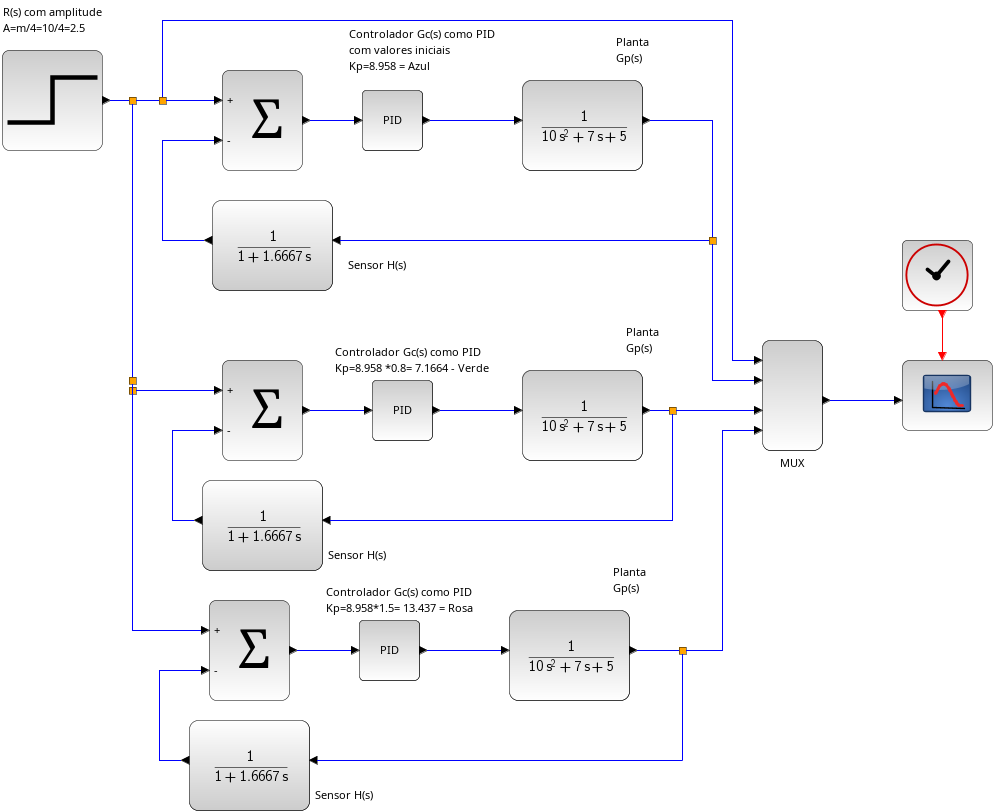
\includegraphics[width=0.8\textwidth]{6-atividade/assets/c/diagrama-pid-ajustando-kp.png}
    \caption{Diagrama de resposta do sistema com diferentes valores de \( K_p \).}
    \label{fig:diagrama-comparacao-proporcional-pid}
\end{figure}

\begin{figure}[H]
    \centering
    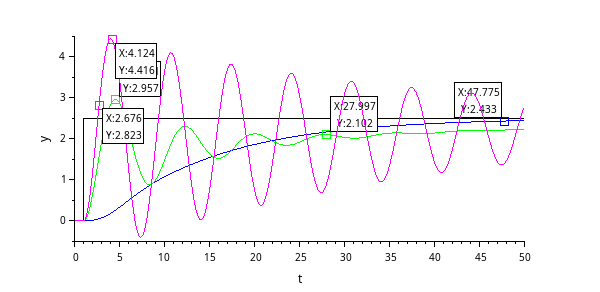
\includegraphics[width=0.8\textwidth]{6-atividade/assets/c/pid-ajustando-kp.png}
    \caption{Resposta do sistema para o \( K_p \) ajustado em comparação com outros valores.}
    \label{fig:comparacao-proporcional-pid}
\end{figure}

\subsubsection{Discussão dos Resultados e Escolha de \( K_p \)}
A análise das respostas mostrou que a redução de \( K_p \) para 7.1664 (80\% do valor inicial) oferece uma melhoria significativa em termos de controle de overshoot e estabilidade do sistema. Este ajuste resulta em uma resposta onde o overshoot é notavelmente menor, o que é vantajoso para sistemas que requerem estabilidade rápida sem oscilações excessivas.

\vspace{0.4cm}
\textbf{Vantagens:}
\begin{itemize}
    \item \textbf{Menor Overshoot:} Redução significativa no overshoot, proporcionando uma resposta mais suave e estável. Essa característica é particularmente benéfica para aplicações que não podem tolerar grandes desvios temporários de suas variáveis de processo.
    \item \textbf{Tempo de Acomodação Razoável:} O sistema atinge o estado estacionário mais rapidamente, o que é crucial para aplicações que demandam respostas rápidas e precisas. Isso é conseguido sem induzir instabilidade prolongada.
\end{itemize}

\vspace{0.4cm}
\textbf{Desvantagens:}
\begin{itemize}
    \item \textbf{Comprometimento da Rapidez Inicial:} A resposta inicial é ligeiramente mais lenta, o que pode não ser ideal para todos os tipos de aplicações, especialmente aquelas que dependem de uma atuação rápida após uma mudança de condições.
    \item \textbf{Sensibilidade a Distúrbios:} A redução do \( K_p \) pode diminuir a capacidade do sistema de reagir eficientemente a perturbações súbitas ou variações significativas na entrada, podendo resultar em um desempenho subótimo sob condições de carga variável.
\end{itemize}

Foi analisado da possibilidade de redução adicional de \( K_p \) diminuir ainda mais \( K_p \) além de 80\% poderia potencialmente levar a uma resposta demasiadamente lenta, comprometendo a capacidade do sistema de reagir a alterações rápidas. Essa mudança requer uma análise cuidadosa das prioridades do sistema: estabilidade versus rapidez de resposta.

\subsubsection{Implementação e Avaliação Futura do Novo \( K_p \)}
O novo \( K_p \) de 7.1664 será implementado no controlador PID para uso continuado. Este ajuste será acompanhado de monitoramento e avaliação contínuos para assegurar que ele atende às exigências do sistema em variadas condições operacionais.

A decisão de ajustar o \( K_p \) para 7.1664 reflete um compromisso bem fundamentado entre resposta rápida e controle de oscilações, adequado para muitas aplicações industriais e de automação. Avaliações futuras focarão em refinamentos adicionais e na otimização de \( K_i \) e \( K_d \) para maximizar a eficácia do sistema de controle.
